%%% Local Variables:
%%% TeX-engine: xelatex
\documentclass{ucetd}

% general
\usepackage{fontspec}
\usepackage{xeCJK}
\usepackage{titlesec}
\usepackage{subfigure,epsfig,amsfonts}
\usepackage{amsmath}
\usepackage{amssymb}
\usepackage{mathrsfs}
\usepackage{wrapfig}
\newenvironment{figurewrap}
 {%
%  \setlength{\intextsep}{0pt}% <--- Wrong!
  \setlength{\columnsep}{15pt}%
  \wrapfloat{figure}%
 }
 {\endwrapfloat}
\usepackage{graphicx}
\usepackage{tikz,pgf}
\usetikzlibrary{backgrounds}
\usepackage{booktabs}
\usepackage{wasysym}
\usepackage{multicol}
\usepackage[linesnumbered,lined,boxed,commentsnumbered]{algorithm2e}
\usepackage{capt-of}
\usepackage{caption}
\usepackage{float}
\usepackage[dvipsnames]{xcolor}
\usepackage{soul}
\usepackage{empheq}
\usepackage{enumitem}
\usepackage[many]{tcolorbox}
\usepackage[
  left=1.35in,
  textwidth=5.9in,
  includeheadfoot,
  voffset=0.5em,
  headsep=1.0em,
  headheight=1.5em,
  textheight=635pt,
  footskip=3.0em
  ]{geometry}% http://ctan.org/pkg/geometry
\setlength{\intextsep}{1.5em}
\setlength{\abovedisplayskip}{-2.0em}
\setlength{\belowdisplayskip}{-2.0em}
\setlength{\abovedisplayshortskip}{-2.5em}
\setlength{\belowdisplayshortskip}{-2.5em}
\setlength{\belowcaptionskip}{0.0em}

% require: amsmath, xcolor, soul, empheq, [many]tcolorbox
% highglighting text
\definecolor{mygreen}{rgb}{0.51, 0.94, 0.63}
\newcommand{\hll}[1]{\colorbox{mygreen}{$\displaystyle #1$}}
\tcbset{
  highlight math style={
    colback=mygreen,
    arc=0pt,
    outer arc=0pt,
    boxrule=0pt,
    top=2pt,
    bottom=2pt,
    left=2pt,
    right=2pt,
  }
}

% encircling numbers
\newcommand*\circled[1]{\tikz[baseline=(char.base)]{
    \node[shape=circle,draw,inner sep=2pt] (char) {#1};}}

% for embedding svg figures made with inkscape
\usepackage{svg}
% frames
\usepackage{framed}

\makeatletter
\newcommand\notsotiny{\@setfontsize\notsotiny\@vipt\@viipt}
\makeatother

\titlespacing{\chapter}{0pt}{-80pt}{1cm}
\titlespacing{\paragraph}{0pt}{0em}{0.8em}

% theorem environments
\usepackage{amsthm, thmtools}

% headers
\usepackage{fancyhdr}
\pagestyle{fancy}
\fancyhead[L]{\rightmark}
\fancyhead[R]{\thepage}
\renewcommand{\headrulewidth}{0pt}

%% subsubsections
\setcounter{secnumdepth}{3} % how many sectioning levels to assign numbers to
\setcounter{tocdepth}{3}    % how many sectioning levels to show in ToC
\newcounter{subsubsection}[subsection]

% references
\usepackage[colorlinks = true,%
linkcolor = black,%
urlcolor  = black,%
citecolor = black,%
anchorcolor = black]{hyperref}
\usepackage{cleveref}

% Bibliography
\usepackage[
    backend    =      biber,%
    style      = authoryear,%
    sortlocale =      en_GB,%
    url        =      false,% 
    doi        =       true,%
    eprint     =      false]{biblatex}
\addbibresource{refs.bib}

% glossary functions
% \usepackage[toc]{glossaries}
% uncomment to make glossary words bold
% \renewcommand*{\glstextformat}[1]{\textbf{#1}}

\newfontfamily\quotefont[ligatures=TeX]{Optima}
\DeclareTextFontCommand{\textquotefont}{\normalfont\quotefont}
\newcommand{\authorquote}[2]{
\begin{center}\begin{quote}
\parbox{0.25cm}{\Large{``}}{\small{\textquotefont{{#1}}}}$\,$\parbox{0.25cm}{\Large{''}} \vspace{-1.30em}\flushright{\small{\textquotefont{{#2}}}}
\end{quote}\end{center}
\vspace{-0.60em}
}
\newcommand{\basicquote}[1]{
\begin{center}\begin{quote}
\parbox{0.25cm}{\Large{``}}{\small{\textquotefont{{#1}}}}$\,$\parbox{0.25cm}{\Large{''}}
\end{quote}\end{center}
}

\usepackage[framemethod=TikZ]{mdframed}
\usetikzlibrary{calc}

\makeatletter
\newrobustcmd*\mdf@tikzbox@tfl@spare[1]{%three or four borders
    \clip(0,0)rectangle(\mdfboundingboxwidth,\mdfboundingboxheight);%
    \begin{scope}[mdfcorners]%
       \clip[preaction=mdfouterline]%
            [postaction=mdfbackground]%
            [postaction=mdfinnerline]#1;%
    \end{scope}%
    \path[mdfmiddleline,mdfcorners] ($(O|-P)-(0,0.25cm)$)--(O|-P)--(P)--($(P)-(0,0.25cm)$);
    \path[mdfmiddleline,mdfcorners] ($(P|-O)+(0,0.25cm)$)--(P|-O)--(O)--($(O)+(0,0.25cm)$);
  }%
\newrobustcmd*\changelinestyle{\let\mdf@tikzbox@tfl\mdf@tikzbox@tfl@spare}
\makeatother


% theorem styles
\declaretheoremstyle[%
headfont=\sffamily\bfseries,%
notefont=\mdseries\itshape\sffamily,%
notebraces={}{},%
headpunct=,%
bodyfont=\sffamily,%
headformat=\NAME~\NUMBER~--\NOTE\hfill\smallskip\linebreak,%
preheadhook=\begin{leftbar},%
  postfoothook=\end{leftbar},%
]{customDefinition}
\declaretheoremstyle[%
  spaceabove=2pt, spacebelow=5pt,
  headfont=\bfseries,
  postheadspace=1.4em,
  notefont=\normalfont\itshape, notebraces={(}{)},
  bodyfont=\normalfont,
]{example}

% theorem environments
\declaretheorem[name=Definition,
style=customDefinition,
numberwithi=chapter,
refname={definition,definitions},
Refname={Definition,Definitions}]{definition}
\declaretheorem[name=Note,
style=definition,
numberwithin=chapter,
refname={note,notes},
Refname={Note,Notes}]{note}
\declaretheorem[name=Example,
style=example,
numberwithin=chapter,
refname={example,examples},
Refname={Example,Examples}]{example}
\declaretheorem[name=Example,
style=example,
numberwithin=chapter,
refname={example,examples},
Refname={Example,Examples}]{example*}
\definecolor{mygrey}{rgb}{0.92, 0.92, 0.92}
\mdfdefinestyle{infobox}{%
  backgroundcolor=white,
  roundcorner=0.7pt,%
  middlelinewidth=0.7pt,%
  skipabove=10pt,%
  splittopskip=1.5em,%
  firstextra={\draw[dashed,line width=0.7pt,xshift=0.7pt] (O) -- (P|-O);},%
  secondextra={\draw[dashed,line width=0.7pt,xshift=-0.7pt] (O|-P) -- (P);},%
  middleextra={\draw[dashed,line width=0.7pt,xshift=0.7pt] (O) -- (P|-O);\draw[dashed,line width=0.7pt,xshift=-0.7pt] (O|-P) -- (P);},%
}

\newenvironment{infobox}[1]%
{\begin{mdframed}[%
    style=infobox,%
    frametitle={\mdseries\sffamily Summary: \vphantom{$frac{1}{2}$}#1},%
    skipabove=\baselineskip plus 3pt minus 1pt,%
    skipbelow=\baselineskip plus 3pt minus 1pt,%
    linewidth=0.5pt,%
    frametitlerule=true,%
    frametitlebackgroundcolor=mygrey]
  }
  {\end{mdframed}}

\surroundwithmdframed[settings=%
\changelinestyle,%
middlelinecolor=black,%
roundcorner=0.7pt,%
middlelinewidth=0.7pt,%
skipabove=10pt,%
splittopskip=1.5em,%
  firstextra={\draw[white, dashed,line width=1pt,xshift=0.7pt, pattern= on 3pt off 3pt] (O) -- (P|-O);},%
  secondextra={\draw[white, dashed,line width=1pt,xshift=-0.7pt, pattern= on 3pt off 3pt] (O|-P) -- (P);},%
  middleextra={\draw[white, dashed,line width=1pt,xshift=0.7pt, pattern= on 3pt off 3pt] (O) -- (P|-O);\draw[dashed,line width=0.7pt,xshift=-0.7pt] (O|-P) -- (P);},%
]{example}
\surroundwithmdframed[settings=%
\changelinestyle,%
middlelinecolor=black,%
roundcorner=0.7pt,%
middlelinewidth=0.7pt,%
skipabove=10pt,%
splittopskip=1.5em,%
  firstextra={\draw[white, dashed,line width=1pt,xshift=0.7pt, pattern= on 3pt off 3pt] (O) -- (P|-O);},%
  secondextra={\draw[white, dashed,line width=1pt,xshift=-0.7pt, pattern= on 3pt off 3pt] (O|-P) -- (P);},%
  middleextra={\draw[white, dashed,line width=1pt,xshift=0.7pt, pattern= on 3pt off 3pt] (O) -- (P|-O);\draw[dashed,line width=0.7pt,xshift=-0.7pt] (O|-P) -- (P);},%
]{example*}

\renewenvironment{leftbar}{%
  \def\FrameCommand{{\vrule width 3pt} \hspace{10pt}}%
  \MakeFramed {\advance\hsize-\width \FrameRestore}}%
{\endMakeFramed}


\institution{University of York}
\title{Word Embeddings}
\author{Joel Strouts}
\date{2021}
\abstract{\noindent
  %% TODO: rewrite
In this report we attempt to provide a comprehensive primer on key topics relating to word embeddings, sufficient to enable further reading of more advanced material. The reader does not need prior experience in the domain of natural language processing (NLP), but familiarity with core mathematics at an undergraduate level is assumed. We take a more cross-disciplinary approach than purely mathematical one to reflect the primarily applied nature the subject matter. In the first chapter we summarise the key features of word embeddings: What they are, how they are created, what they are for, and other uses the theory of word embeddings outside of NLP. In the second chapter we discuss the difficulties of defining word meaning and present a framework to help distinguish between different senses of `word'. In the third chapter we describe key concepts and definitions generally assumed by the different methods for generating word embeddings. Finally in the fourth chapter we illustrate these ideas by describing the operation of particular class of embedding methods: count models.}

\begin{document}

\maketitle

\mainmatter{%
\tableofcontents
\chapter{Introduction}
\section{What are word embeddings?}
Word embeddings are numerical representations of words which are derived from the observed patterns of word usage in a body of example text. These representations take the form of position vectors within a \textit{Word Space}. The resulting \emph{Word Space Model} was first described by \textcite{shutze-1993-word-space} in the terms:
\basicquote{\noindent
  [The Word Space Model] uses feature vectors to represent words, but the features cannot be interpreted on their own. Vector similarity is the only information present in Word Space: semantically related words are close, unrelated words are distant.}
\begin{example}[Two Dimensional Word Space]\label{ex:2d-word-space}
  \noindent
  The word space in \autoref{fig:2d-wvs} illustrates both components of the above definition: first that related words are closer in space than less related words (the words \textit{apple} and \textit{orange} are closer in space than \textit{apple} and \textit{bicycle}), and second that the individual axis of variation are not meaningful considered in isolation from one another (there is no trait like `size'  which the $x$ or $y$ value for a word is descriptive of).
  \begin{figure}[H]
    \centering
    \begin{minipage}[t]{.4\textwidth}
      \centering
      \vspace{0.4em}
      \begin{tikzpicture}[scale=1.4]
        \draw[<->, very thick] (-2,0) -- (2,0);
        \draw[<->, very thick] (0,-2) -- (0,2);
        %% \draw[steps=.25cm,gray,very thin] (-4,-4) grid (4,4);
        \node at (-1.55 , -0.45 ) {red};
        \node at (-1.35 , -1.00 ) {orange};
        \node at ( 0.63 ,  1.50 ) {monday};
        \node at ( 1.3  ,  1.10 ) {tuesday};
        \node at ( 0.7  , -0.75 ) {bicycle};
      \end{tikzpicture}
      \caption{A two dimensional word space encoding semantic information about the five words; \emph{red, orange, monday, tuesday \& bicycle}}\label{fig:2d-wvs}
    \end{minipage}\hspace{4em}
    \begin{minipage}[t]{.4\textwidth}
      \centering
      \vspace{0.5em}
      \begin{tabular}{l r r}
        \toprule
        \multicolumn{1}{c}{\raisebox{-9pt}[0pt][0pt]{\quad word\quad}} & \multicolumn{2}{c}{features} \\
        \cmidrule(lr){2-3}
        \quad\quad & $x$ & $y$ \\
        \midrule
        red     & -1.55 & -0.45   \\
        orange  & -1.35 & -1.0  \\
        monday  &  0.63 &  1.5   \\
        tuesday &  1.3  &  1.1   \\
        bicycle &  0.7  & -0.75  \\
        \bottomrule
      \end{tabular}
      \vspace{0.42em}
      \captionof{table}{Feature vectors representing the words in \autoref{fig:2d-wvs}}\label{tab:2d-wvs}
    \end{minipage}
  \end{figure}
  \vspace{-0.5em}
\end{example}
More recent research has suggested that word spaces can in fact arrange word-representations with more order than \citeauthor{shutze-1993-word-space}'s early description of these spaces accounted for. Notably, \parencite{mikolov-etal-2013-linguistic} demonstrated their potential for geometrically encoding semantic relationships between words (the \emph{direction} in which one vector is distant from another can capture semantic information, not only the distance). \autoref{fig:word-space-geometry} illustrates the idea of geometrically encoded semantic information. Indeed, modern methodologies for assessing the quality of a word space consider the extent to which \emph{multifaceted} linguistic information about the vocabulary (not just semantic, but; phonetic, morphological, and syntactic information about the encoded words) is recoverable by the embeddings \parencite{yaghoobzadeh-schutze-2016-intrinsic, wang-2019-evaluating}.
\begin{figure}[H]
  \captionsetup{width=.91\linewidth}
  \centering
  \begin{minipage}[t]{.40\textwidth}
    \centering
    \begin{tikzpicture}[framed,scale=1.15]
      \node at ( -2  , 0) {man};
      \node at (  0  , 2) {woman};
      \draw[->, very thick, blue] (-2+0.3, 0+0.3) -- (0-0.3, 2-0.3);
      \node at (-2 , 1.5) {uncle};
      \node at ( 0 , 3.5) {aunt};
      \draw[->, very thick, blue] (-2+0.3, 1.5+0.3) -- (0-0.3, 3.5-0.3);
      \node at (-4.5 , 2 ) {king};
      \node at (-2.5 , 4 ) {queen};
      \draw[->, very thick, blue] (-4.5+0.3, 2+0.3) -- (-2.5-0.3, 4-0.3);
    \end{tikzpicture}
  \end{minipage}\hspace{3.5em}
  \begin{minipage}[t]{.40\textwidth}
    \centering
    \begin{tikzpicture}[framed,scale=1.15]
      \node at ( -2  , 0) {man};
      \node at (  0  , 2) {woman};
      \draw[->, very thick, blue] (-2+0.3, 0+0.3) -- (0-0.3, 2-0.3);
      \node at (-4.5 , 2 ) {king};
      \node at (-2.5 , 4 ) {queen};
      \draw[->, very thick, blue] (-4.5+0.3, 2+0.3) -- (-2.5-0.3, 4-0.3);
      % man -> king
      \draw[->, very thick, red] (-2-0.38, 0+0.30) -- (-4.5+0.38, 2-0.30);
      % woman -> queen
      \draw[->, very thick, red] ( 0-0.38, 2+0.30) -- (-2.5+0.38, 4-0.30);
    \end{tikzpicture}
  \end{minipage}
  \caption{An idealised illustration of how semantic \& syntactic information could be geometrically encoded by embeddings in a word space\footnotemark.}\label{fig:word-space-geometry}
\end{figure}}%
\footnotetext{We use the term \emph{idealised} here because although this figure is a reproduction of that which accompanies the famous $\overrightarrow{\text{king}}-\overrightarrow{\text{man}}+\overrightarrow{\text{woman}}=\overrightarrow{\text{queen}}$ example from~\parencite{mikolov-etal-2013-linguistic}, more recent investigations \parencite{linzen-2016-issues, rogers-etal-2017-many} have concluded that these analogical relationships are not the \emph{robust} features of word space geometry suggested by these figures. Nevertheless, investigations into the geometry of word space have found some notable structure \parencite{liu-2018-visual-explor}.}\noindent
Typical word spaces, unlike the simplified form illustrated in \autoref{ex:2d-word-space}, are \emph{high-dimensional}: it is common for the dimension of a word space to be in the order of tens, hundreds, or thousands. In a relatively low-dimensional pre-trained word embedding model\footnote{Model provided by \textcite{pennington2014glove}. Available for download at \href{https://nlp.stanford.edu/projects/glove/}{(GloVe project website)}} the word \emph{orange} (which is represented in the above example by the vector $\text{orange}\mapsto\langle -1.55, 0.35\rangle$) is embedded as the 50-dimensional vector: \vspace{-1.0em}
\begin{align*}
  &\text{orange}\mapsto\\
  \text{\small{$\langle$}}
  &\texttt{\scriptsize ~-0.42783~,~~0.43089~,~-0.50351~,~~0.5776~~,~~0.097786,~~0.2608~~,~-0.68767~,~-0.31936~,~-0.25337~,~-0.37255~,}\\
  &\texttt{\scriptsize ~-0.045907,~-0.53688~,~~0.97511~,~-0.44595~,~-0.50414~,~-0.086751,~-1.0645~~,~~0.36625~,~-0.52428~,~-1.3413~~,}\\
  &\texttt{\scriptsize ~-0.2391~~,~-0.58808~,~~0.56378~,~-0.062501,~-1.7429~~,~-0.88077~,~-0.27933~,~~1.4705~~,~~0.50436~,~-0.69174~,}\\
  &\texttt{\scriptsize ~~2.0018~~,~~0.26663~,~-0.85679~,~-0.18893~,~-0.021125,~-0.055118,~-0.50337~,~-0.67157~,~~0.55502~,~-0.8009~~,}\\
  &\texttt{\scriptsize ~~0.10695~,~~0.1459~~,~-0.55588~,~-0.64971~,~~0.22046~,~~0.67415~,~-0.45119~,~-1.1462~~,~~0.16348~,~-0.62946~}
  \text{\small{$\rangle$}}\tag{\theequation}\label{eq:orange-vec}\vspace{-1.0em}
\end{align*}
High-dimensional vectors like \eqref{eq:orange-vec} cannot be plotted on an $x,y$ plane without loss of information, so we can't visualise points in a typical word space with the same approach as we used in \autoref{ex:2d-word-space}. An alternate method for visualising points in word space which still allows us to judge the similarity of vectors by their appearance, and is applicable higher dimensional vectors, is to map the magnitude of vector components onto a smooth colour gradient and then to compare the resulting colour-vectors, rather than the original numerical forms.
\begin{example}[50 dimensional Word Space]\label{ex:glove-word-space}%% todo: expand on this description
\autoref{fig:glove-word-space} applies the principle described above to visualise word vector outputs from a real word embedding model. Each row of coloured cells represents the word vector for the word to its left. More negative entries are more blue, and more positive entries are more red. You can see, for example, that the vectors for \emph{monday} and \emph{tuesday} are very similar to one another, whereas the vectors for \emph{tuesday} and \emph{bicycle} are very different.
\begin{figure}[H]%% add key to figure
  \captionsetup{width=.91\linewidth}
 \centering
 \includesvg[width=0.91\linewidth]{figures/python/wiki_vecs.svg}
 \caption{A selection of embeddings from the same pre-trained 50-dimensional \emph{GloVe} word space model from which the \emph{orange} vector in \eqref{eq:orange-vec} was taken.}\label{fig:glove-word-space}
 \centering
\end{figure}
\end{example}

\section{How are they created?}
Word embeddings are the output of \emph{word embedding algorithms}: Processes which take as their input large body of example language-usage and \emph{automatically produce} (i.e., without need for further instruction from the practitioner) representations of the observed words \emph{which encode a means of quantifying the semantic-relatedness of those words}.
\authorquote{What makes the word-space model unique in comparison with other geometrical models of meaning is that the space is constructed with no human intervention, and with no a priori knowledge or constraints about meaning similarities. In the word-space model, the similarities between words are automatically extracted from language data by looking at empirical evidence of real language use.}{\textcite{sahlgreen-2006-the-word-space-model}}
How exactly is this information automatically extracted from a corpora of ``real language usage'' though? \citeauthor{sahlgreen-2006-the-word-space-model} continues:
\basicquote{As data, the word-space model uses statistics about the distributional properties of words. The idea is to put words with similar distributional properties in similar regions of the word space, so that proximity reflects distributional similarity. The fundamental idea behind the use of distributional information is the so-called distributional hypothesis.}
\begin{definition}[The Distributional Hypothesis]
There are many variations of the statement of the distributional hypothesis; \citeauthor{sahlgreen-2006-the-word-space-model} opts for the more general phrasing \emph{``words with similar distributional properties have similar meanings''}, but with reference to its application in creating word spaces cites the more concrete \emph{``words with similar meanings will occur with similar neighbours if enough text material is available''} of \textcite{schutze-1995-information-retrieval} and the concise \hll{\emph{``words which are similar in meaning occur in similar contexts''}} of \textcite{rubenstein-1965-contextual-correlates}. \textcite{firth-1957-a-syn-of-lin} notably captured the essence of this hypothesis with the much quoted statement \emph{``You will know a word by the company it keeps''}.
\end{definition}\label{def:distrib-hyp}
\begin{example}[The distributional hypothesis]
  In the figure from~\autoref{ex:glove-word-space}, the vector representations of the words ``Monday'' and ``Tuesday'' are almost identical to one another. These representations were generated by analysing the contexts each word occurred in, so implied by this result is that the words ``Monday'' and ``Tuesday'' occur in very similar contexts. Consider these partial quotations\footnotemark:
  \begin{align}
    &\text{``I'd be quite happy if I spent from Saturday night until \underline{~~~~~~~~~~} morning\dots''}\label{eq:distrib-hyp-1}\\
    &\text{``It was a \underline{~~~~~~~~~~} and they walked on a tightrope to the sun.''}\label{eq:distrib-hyp-2}\\
    &\text{``I will love you at 4:15 pm next \underline{~~~~~~~~~~}.''}\label{eq:distrib-hyp-3}\\
    &\text{``\dots the kind that blindside you at 4 pm on some idle \underline{~~~~~~~~~~}.''}\label{eq:distrib-hyp-4}
  \end{align}
  In each of these contexts one can infer that the \emph{type} of word which is missing is likely to be a day of the week, but it is difficult to guess with confidence any more specifically; the words ``Monday'' and ``Tuesday'' seem to be almost equally probable guesses -\emph{their similarity of meaning is reflected in the similarity of their contexts}.
\end{example}
\footnotetext{These quotations were found by searching for quotes containing the word ``Monday'' (in the case of~\eqref{eq:distrib-hyp-1} and~\eqref{eq:distrib-hyp-2}) or ``Tuesday'' (in the case of~\eqref{eq:-distrib-hyp-3} and~\eqref{eq:distrib-hyp-4}) on the \href{https://www.goodreads.com}{goodreads} website}
This \emph{distributional} linguistic perspective was widespread in the 1950s \parencite{jurafsky21-speec}, with key contributions to the theory made by \textcite{joos-1950-description-of-language, harris-1954-distrib-struct, firth-1957-a-syn-of-lin}, and is related \citeauthor{wittgenstein53-philos}'s \parencite*{wittgenstein53-philos} ideas about `family resemblance' from the same period \parencite{turney10-from-frequen-to-meanin}.

The question of how word embeddings are created can then instead be phrased \emph{How exactly is the distributional hypothesis employed by these (word embedding) algorithms?}. Below we paraphrase the descriptions of seven notable classes of word embedding methods, due to \textcite{wang-2019-evaluating}:
\begin{infobox}{Word Embedding Method Categorisation}
  \paragraph{*Co-occurrence Matrix}\label{cooccurrence-matrix-models} These methods work by building a matrix which counts the number of time each word co-occurs within a particular context. Different versions define different meanings of ``context''  (\textcite{turney10-from-frequen-to-meanin, sahlgreen-2006-the-word-space-model} provide a good overview of approaches).
  \paragraph{Continuous-Bag-of-Words and skip-gram}\label{word2vec-models} Two \emph{iteration-based} neural network methods proposed in the \texttt{word2vec} paper \parencite{mikolov13-effic-estim-word-repres-vector-space} and widely used thereafter. The first model (CBOW) predicts the center word from its surrounding context and the second (SG) predicts the surrounding context words given a center word.
  \paragraph{Neural Network Language Model}\label{nnl-model} The NNLM~\parencite{bengio-2003-a-neural-prob-lang-model} \emph{jointly learns a word vector representation and a statistical language model}, and is ``very computationally complex''.
  \paragraph{FastText}\label{fasttext} This method exists to address issues with other approaches which produce poor estimations for rarely used words. ``FastText uses subword information explicitly so embedding for rare words can still be represented well''. It is based on the skip-gram model, where each word is represented as a bag of character 
  \paragraph{$N$-gram Model}\label{n-gram-model} $n$-grams are multi-word elements with $n$ parts (for example ``a man'' is a 2-gram). $n$-gram models are methods which operate on $n$-grams in addition to, or in place of words. \textcite{zhao-etal-2017-ngram2vec} incorporates the n-gram model in various baseline embedding models such as \texttt{word2vec}, GloVe, PPMI, and SVD.
  \paragraph{Dictionary Model}\label{dictionary-model} Dictionary models learn word representations from dictionary entries as well as large unlabelled corpus, both sources of information are incorporated into one representation. \parencite{tissier-etal-2017-dict2vec} implements this method as \texttt{dict2vec}.
  \paragraph{Deep Contextualised Model}\label{deep-contextualised-model} \parencite{peters18-deep-contex-word-repres} introduced a model for ``deep contextualised word representations which represent complex characteristics of words and word usage across different linguistic contexts''. An \emph{Embeddings from Language Models} (ElMo) representation is generated with by a function which operates on language at the sentence level.
\end{infobox}
In this report we describe algorithms for generating embeddings using the class of methods described here as the \emph{co-occurrence matrix} category (which we refer to as ``count models'').

\section{What are they for?}
\authorquote{The task of representing words and documents is part and parcel of most, if not all, Natural Language Processing (NLP) tasks. In general, it has been found to be useful to represent them as vectors, which have an appealing, intuitive interpretation, can be the subject of useful operations (e.g. addition, subtraction, distance measures, etc) and lend themselves well to be used in many Machine Learning (ML) algorithms and strategies.}{\textcite{almeida19-word-embed}}
Although there are a variety of different word embedding algorithms, each being suited to a different niche of application, they are all united by the following traits:
\begin{infobox}{Shared Characteristics of Word Embedding Algorithms}
\paragraph{Semantic Comprehension} They provide a means of quantitatively assessing the semantic-relatedness of words;
\paragraph{Convenient Form} The semantic information is encoded by \emph{vector} representations of vocabulary words;
\paragraph{Automatic Generation Process} The semantic information is ``\emph{automatically} extracted from language data by looking at empirical evidence of real language use''.
\end{infobox}
The \emph{semantic comprehension} quality makes them appropriate for many tasks in natural language processing, and their \emph{convenient form} (like \citeauthor{almeida19-word-embed} notes above) in particular makes them work well as inputs to machine learning pipelines -\textcite{shutze-1993-word-space} notes: \emph{``Neural networks perform best when similarity of targets corresponds to similarity of inputs; traditional symbolic representations do not have this property''}\footnote{The term ``traditional inputs'' here refers to ``one-hot'' (OH) representations which encode a word with a vector as long as the vocabulary, with all entries zero except for the index corresponding to the place of that word in the vocabulary, which has a value of 1 instead. These vectors contained no information about what words meant, and additionally they were often inconveniently long (as long as the vocabulary).}. Finally, their \emph{automatic generation process} makes them preferable to alternative means of assessing word-relatedness which depend on extensive manual knowledge-input, like building the structured lexical database: \texttt{wordnet} \parencite{miller-1990-intro-to-wordnet}.
\par
\begin{figurewrap}[10]{r}{0.5\textwidth}
  \vspace{-3.5em}
  \captionsetup{width=.4\textwidth}
  \centering
  \includesvg[width=.5\textwidth]{figures/python/wiki_vecs_dendogram.svg}
  \caption{Word clusters identified by analysis of word vectors featured in \autoref{fig:glove-word-space}}\label{fig:glove-word-clusters}
  \vspace{-10em}
\end{figurewrap}
\par
\textcite{turney10-from-frequen-to-meanin} include a thorough discussion of applications of \emph{Vector Space Models} (the class of embedding algorithms referred to as \emph{count models} in this report), listing the following examples of uses: word clustering, word classification, automatic thesaurus generation, word sense disambiguation, context sensitive spelling correction, semantic role labelling, query expansion, textual advertising \& information extraction. \Cref{fig:glove-word-clusters} illustrates the use of the embeddings from \autoref{fig:glove-word-space} to perform the first task from this list of examples: automatic word clustering.

Word embeddings do not have a predefined list of applications of course, they can be used as a tool any way that can be imagined for them. Novel applications we have come across in our research include: detecting signs of dementia \parencite{mirheidari-2018-detecting-signs-of-dementia}, learning representations of medical concepts \parencite{ChoiChiuSon-amia16}, to investigate the nature of human language acquisition \parencite{landauer-1997-a-solution}, \& to map the changing biases encoded by language over the span of a century \parencite{garg-2018-word-embeddings-quantify}.

\begin{example}[Word Clustering Using Embeddings]\label{ex:glove-word-clusters}
  \autoref{fig:glove-word-clusters} shows the result of using a point-clustering algorithm on the embeddings from \autoref{fig:glove-word-space} to identify groups of related words. The resulting clusters, identified entirely computationally, correspond with the groupings an English speaker would naturally select given the same word choices.
\end{example}


\section{Beyond word embeddings}\label{chap:beyond-word-embeddings}
Word embedding algorithms extract semantic information about language without `knowing' what language is. To these algorithms, language is just lists of discrete elements with underlying patterns to be identified. Due to this generality, word embedding algorithms can be used to encode the semantics of other types of ordered data.
Many novel applications of the embedding process to capture semantic associations outside of the written language domain have been explored. Below we list some notable embedding applications we have come across in researching for this report:
\par
\begin{infobox}{Novel Applications of the Embedding Process}
  \paragraph{Graph Embeddings} \textcite{grohe20-word2-node2} presents an overview of techniques which generalise the word embedding process to embed structured data -graphs (possibly labelled or weighted), or more generally relational structures, nodes of a large graph, or tuples appearing in a relational structure.
  \paragraph{Recommendation Systems} \textcite{grbovic-2018-real-time-personalization} demonstrate the use of \emph{user} and \emph{listing} embeddings to improve real-time personalisation and ``similar listing" recommendations at Airbnb, and \textcite{wang-2018-billion-scale-commodity-embedding} employ item-graph embeddings generated from users' behaviour history to improve recommendation systems at the global e-commerce platform Alibaba.
  \paragraph{Music Embeddings} \textcite{chuan-2018-from-context-to} model functional chord relationships and harmonic associations by embedding slices of music from a large corpus music across eight genres.
  \paragraph{Customer Lifetime Value Prediction} \textcite{chamberlain17-custom-lifet-value-predic-using-embed} propose a method to generate embeddings of customers which provide daily estimates of the future value of every customer, employed by the ASOS fashion retailer.
\end{infobox}
While the focus of this document is on the use of embeddings to process language, it is our intention to present the theory of word embeddings in such a way that the underlying techniques \emph{not specific to language processing} can be understood in their own right. We intend that novel applications like those mentioned above, falling outside of the field of NLP, can be approached with proper context following this primer.

\section{Report Content \& Structure}
%% TODO: state key references (turney.. mikolov etc.)
In \autoref{chap:words} we discuss words themselves: what are they and what does it mean to represent them? In \autoref{chap:words} we present key concepts and definitions necessary to make sense of the details of the different word embedding processes. In \autoref{chap:count-models} we describe two describe two methods for creating word spaces, one based on documents and one based on context-windows. Once we have presented these count-based embedding methods we compare their qualities to those of other possible approaches. Finally we provide references for \nameref{chap:further-reading} and make closing remarks on the content \& concepts presented in this report in the \nameref{conclusion}.
%% -------------------------- %%
%%        MAIN MATTER         %%
%% -------------------------- %%
\chapter{Words}\label{chap:words}
\newsection{What are words?}
\authorquote{To many people the most obvious feature of a language is that it consists of words}{\textcite{halliday-2004-lexicology}}
\authorquote{There have been many definitions of the word, and if any had been successful I would have given it long ago, instead of dodging the issue until now}{\textcite{matthews-1991-morph}}
\noindent
The `Word' workshop, held at the international research centre for linguistic typology 12-16 August 2000 consisted of 16 presentations discussing the answer to this question. Ten of those were published in the book \citetitle{dixon02-word}. The difficulty of the question is summarised in the book's conclusion as follows:
\authorquote{The problem of the word has worried general linguists for the best part of a century. In investigating any language, one can hardly fail to make divisions between units that are word-like by at least some of the relevant criteria. But these units may be simple or both long and complex, and other criteria may establish other units. It is therefore natural to ask if ‘words’ are universal, or what properties might define them as such.}{P.H. Matthews, \parencite{dixon02-word}}
\noindent
Some definitions of 'word' (like \citeauthor{bloomfield-1926-a-set-of}'s \parencite*{bloomfield-1926-a-set-of} \emph{`A minimum free form is a word'}) are sufficient but not necessary, wheras others (like \citeauthor{lyons-1968-introduction}'s \parencite*{lyons-1968-introduction} \emph{`a word may be defined as the unit of a particular meaning with a particular complex of sounds capable of a particular grammatical employment'}) is a potentially necessary, but certainly not sufficient \parencite{dixon02-word}. Is it possible to conceive a watertight definition?

Our intuition about words is also often inscrutible -consider \emph{so called} filler-words like ``uh'' or ``um'', or compound forms like ``rock `n' roll'' and ``New York'', used always as whole unbroken units, what makes these \emph{not} words? Consider that the words we agree on now are subject to ever changing convention; the word ``tomorrow'' is listed in Johnson's 1755 dictionary of the English language as two distinct components ``to'', and ``morrow'' despite being indisputably considered a word \emph{to-day}. \textcite{halliday-2004-lexicology} ask ``How do we decide about sequences like lunchtime (lunch-time, lunch time), dinner-time, breakfast time? How many words in isn't, pick-me-up, CD?''.

An understanding of `word' formed within the English language cannot blindly be applied beyond that scope either, \textcite{dixon02-word} notes ``The idea of `word' as a unit of language was developed for the familiar languages of Europe''. Languages which are written without spaces, (like Chinese, Japanese, and Thai) present one particular example of the challenges in applying a local conception of `word' beyond this scope: ambiguous sentence segmentation. 
\begin{example}[Chinese Sentence Segmentation]
  \textcite{chen-2017-adversarial-multi} gives the following example of the difficulty in agreeing on `word' boundaries in Chinese: The sentence "Yao Ming reaches the finals" (姚明进入总决赛) May be divided up to yield either three words or five using the two segmentations methods; `Chinese Treebank' segmentation, or `Peking University' segmentation, respectively:
  \begin{align*}
    &\texttt{姚明~~~~~进入~~~~~总决赛~}\\\tag{Chinese Treebank}
    &\texttt{YaoMing~~reaches~~finals}\\
    \\
    &\texttt{姚~~~明~~~~进入~~~~~总~~~~~~~决赛}\\\tag{Peking University}
    &\texttt{Yao~~Ming~~reaches~~overall~~finals}
  \end{align*}
\end{example}
Different languages present different difficulties -In the case of Arabic, expressions formed by adding consecutive suffixes to a single root word (like the sequence \emph{establish $\to$ establishment $\to$ establishmentarianism} in English) are a more essential part of the language, such that complete sentences can be expressed as unbroken `word' units. As a result a `word' unit, which is identified by unbroken character sequences occuring between spaces, in Arabic will represent larger more complex chunks of meaning than same framework would identify for comparable sentences in English. What is the `correct' amount of information that our word-units should encode?
\section{A `word' framework}
\authorquote{There is a general concept underlying all this diversity; that is the \textbf{lexical item}. Every language has a \textbf{vocabulary}, or 'lexicon', which forms one part of its grammar —or, to use a more accurate term, one part of its lexicogrammar}{\textcite{halliday-2004-lexicology}}
To clarify what is meant by `word' beyond just a description of convetion requires a new vocabulary: we need terms which allow us to describe the various commonalities of form and function which unify of these elements of everyday language. We present a framework due to \textcite{dixon02-word} to assist us toward this end:
\begin{infobox}{Distinguishing between uses of the term \emph{word} \parencite{dixon02-word}}
  The word `word' is used in many ways in everyday speech, and in much linguistic discourse. It is important to make certain fundamental distinctions:
  \begin{enumerate}[label=\protect\circled{\small{\arabic*}}]
    \item Between a lexeme and its varying forms;
    \item Between an orthographic word (something written between two spaces) and other types of word;
    \item Between a unit primarily defined on grammatical criteria and one primarily defined on phonological criteria.
  \end{enumerate}
\end{infobox}
Let us briefly clarify what is meant by these terms before discussing their relevance to word embeddings:
\begin{definition}[Lexemes and inflected forms]
  Lexemes are distinct \emph{root forms} which make up the \emph{lexicon} of a language (they are the elements of which dictionaries generally constitute), and serve to group so-called \emph{inflected forms} which have a meaning related to their root. Lexemes are the object being referred to as `word' in statements like ``look, looks, looked and looking are forms of the same word''. The same sentiment could be phrased: ``the lexeme \emph{look} is realised as the word-forms: \emph{look, looks, looked \& looking}''.
\end{definition}
\begin{example}[Lexemes and inflected forms]\label{ex:lexemes}
  The example given above of contrasting the lexeme ``look'' to its inflected forms is presented here in a table:
  \begin{table}[H]
    \centering
    \begin{tabular}{l l l l}
      \toprule
      root or underlying form & inflected forms & grammatical function\\
      \midrule
      look                    & look            & present, non-3sg subject\\
                              & looks           & present, 3sg subject\\
                              & looked          & past\\
                              & looking         & participle\\
      \bottomrule
    \end{tabular}
    \caption{An comparison between the lexeme for the English verb \emph{look} and its inflected word-form realisations}
  \end{table}
\end{example}
\vspace{1em}
\begin{definition}[Orthographic words]
  Orthographic words are distinct elements of \emph{orthography} (written language), most often defined as \textbf{something written between two spaces}.
\end{definition}
\begin{example}[Orthographic words]\label{ex:orthographic-words}
  Orthographic words entirely reflect conventions of writing, so the form ``cannot'' is one orthographic word wheras the form ``must not'' (despite having the same apparent grammatical properties) is two orthographic words.
\end{example}
\begin{definition}[Grammatical and phonological words]
  This term describes the language-parts which result from applying a grammatical framework to recognise regular word-like elements in obsereved language. A gramatical framework is one concerned with the rules governing the arrangement of \emph{morphemes} (the smallest distinct units of meaning)
  \textcite{dixon02-word} provides the following criterea for identifying grammatical words:
  A \textbf{grammatical word} consists of a number of gramatical elements which;
  \begin{enumerate}[label=(\alph*)]
  \item always occur together, rather than scattered through the clause (the critereon of cohesiveness);
  \item occur in a fixed order
  \item have a conventionalised coherence and meaning
  \end{enumerate}
  \citeauthor{dixon02-word} also provide a definition of \emph{phonological word} in the same vein which we omit here since phonological words are less directly related to the embedding problem\footnotemark.
\end{definition}
\footnotetext{ Whereas grammatical words are concerned with elements of a grammatical structure with a regular form, phonological words are concrened with elements of a phonological structure (consisting of phonemes: the smallest distinct units of vocalised language) with a regular form. Since word embeddings deal with written language the vocal realisation of language is of less significance.}

\begin{example}[Grammatical words]
  Grammatical words conform less to our conventional notion of `word' but are more well behaved as they derive from a static criterea; The inflected forms of the lexeme \emph{look} in \autoref{ex:lexemes} (\emph{look, looks, looked, looking}) are all examples of grammatical words, but so are the forms ``New York'', ``Rock `n' Roll'', ``dinner-time'', ``breakfast time'', ``isn't'', ``pick-me-up'', and ``CD'' (which we wondered about the proper place of at the start of this chapter). Since the criterea for identifying grammatical words takes meaning into account, different words with the same word-form (like river \emph{bank} and financial \emph{bank}) are also considered distinct grammatical words.
\end{example}
We highlight these distinctions because without this terminology it is easy to overlook an implicit \emph{word}$=$\emph{orthographic word} assumption made when working with word embeddings. This assumption is not uncommon, as \citeauthor{dixon02-word} notes:
\basicquote{In many language communities a word is thought of as having (semantic, grammatical and phonological) unity and, in writing, words are conventionally separated by spaces}
\par
\begin{figurewrap}[13]{r}{0.6\textwidth}
  \vspace{-2.5em}
  \captionsetup{width=.55\textwidth}
  \centering
  \includesvg[width=.60\textwidth]{figures/inkscape/polysemy-figure.svg}
  \caption{The \emph{problem of polysemy} illustrated: Which sense of the orthographic words ``bank'' or ``rock'' should their embeddings encode? and what about the embedding of the grammatical word ``rock `n' roll'' not present in the orthographic words?}\label{fig:polysemy}
\end{figurewrap}
\par
but it is worth discussing explicitly since our assumptions will be encoded by our embedding algorithms. The issues relating most to the generation of word embeddings regard \emph{semantic} unity -if a word does not have semantic unity (i.e., orthographic word and semantic meaning are not one-to-one) then it is said to be \emph{polysemic} (\emph{poly} [many] \emph{semus$\rightarrow$semantic} [meanings]) and the resulting problem w.r.t. word embeddings is called \emph{the problem of polysemy}. A related problem is that of representing grammatical words which consist of multiple orthographic-word parts -these are considered as separate parts and not as a whole.
Ideally word embeddings algorithms would describe a bijective map between grammatical words and points in word space. Since word embedding algorithms operate on orthographic words, the idiosyncrasies of the map between grammatical words and orthographic words (illustrated in \autoref{fig:polysemy} is inhereted by the resulting representations. The surjectivity of this map creates the problem of polysemy and the one-to-many nature of the map means multi-part grammatical words are misrepresented too.
\citeauthor{halliday-2004-lexicology} discuss some of the pitfalls of seeking \emph{fixed, representative} meanings of words in natural lanugage in the following excerpt:
\basicquote{As users of language we know that someone's mention of a recent television programme about big cats in Africa implies a different meaning of cat from a reference to the number of stray cats in the city of New York. And if someone talks about 'letting the cat out of the bag' or 'setting the cat among the pigeons', we know that the meaning has to be taken from the whole expression, not from a word-by-word reading of Felis catus jumping out of a bag or chasing Columbidae. Any good dictionary recognises this by such strategies as listing different senses of a word, giving examples of usage, and treating certain combinations of words (such as idioms) as lexical units. But it is important to recognise that this contextualisation of meaning is in the very nature of language and not some unfortunate deviation from an ideal situation in which every word of the language always makes exactly the same semantic contribution to any utterance or discourse. \textbf{For reasons such as these, we should be cautious about the view that words have a basic or core meaning, surrounded by peripheral or subsidiary meaning(s)}}
Clearly these qualities of language, particularly in its written form, present some difficulties for embedding algorithms. Despite this however, even the earliest embedding methods, which did not take measures to address these concerns, reported that the semantic information they \emph{did} capture was useful and interesting \parencite{deerwester-1990-indexing-by-lsa}.

The embedding methods we present in this report (co-occurence models and \texttt{word2vec} models) do not address the problem of polysemy or the many-to-one problem of multi-part grammatical words, but with the information presented here the reader should: {\small\circled{1}} know the comprimises made by models not accounting for these factors, and {\small\circled{2}} have the context and prerequisites upon finishing this report to understand methods which \emph{do} address the issues. In particular the \nameref{deep-contextualised-model} addresses polysemy concerns, and embeddings operating on n-grams (\nameref{n-gram-model}) address the many-to-one problem.

% ++ words: what are they?
\chapter{Embedding Methods: Preliminaries}
In this chapter we outline briefly terms and distinctions to be used by the embedding algorithms discussed in later chapters.

\section{Types and Tokens}
To process language, it is useful to make the following distinction between two ways of talking about at word-instances, identified by the different ways they are counted:
\begin{definition}[Types and tokens]
  When we count the number of unique vocabulary items in a document we call the things counted \emph{word-types}, whereas when we add up the number of words in a ``word count'' repetitions are permitted and we call the things counted \emph{word tokens}.
\end{definition}
Consider the following example:
\begin{example}[Types and tokens]\par
\phantom{line}
\authorquote{The limits of my language means the limits of my world}{\textcite{wittgenstein-1922-tract}}
This sentence contains $11$ word-tokens, but only $7$ word-types because the four words ``\emph{the limits of my}'' are each repeated once.
\end{example}
This distinction is very useful when processing language, however, as \textcite{kaplan-1990-words} notes, this type/token distinction is very much an \emph{orthographic} construction -this is most straightforwardly apparent in the case of identical tokens which represent separate ``grammatical words'' (like the different grammatical words `rock (music)' and `rock (stone)' both represented by the same orthographic word `rock' in \autoref{fig:polysemy}). \citeauthor{kaplan-1990-words} discusses the shortcomings of this type/token model as a tool for \emph{understanding} language in depth, asserting ``The criterion of word identity is not resemblance'' -however, whether this distinction has \emph{explanatory power} regarding language or otherwise, it inarguably has \emph{utility} when processing language.

\section{Distributional Similarity \& Semantic relatedness}\label{sec:semantic-relatedness}
Up until this point we have used the terms ``semantic relatedness'' and ``word similarity'' interchangeably without clarifying what we are referring to in either case. We have said that word embedding algorithms use observed \emph{distributional similarity} to infer underlying \emph{semantic relatedness/word similarity}, but not discussed the specifics of this inference. In this section we first define a variety of ways in which words can be semantically related, then we discuss types of distributional similarity which can reveal semantic relations, and finally we discuss the limits of this methodology.

We reference \citeauthor{turney10-from-frequen-to-meanin}'s \parencite*{turney10-from-frequen-to-meanin} framework for distinguishing between types of semantic relatedness. First, they describe the general concept of semantic relatedness as follows:

\basicquote{The term semantic relatedness in computational linguistics \parencite{budanitsky-2001-semantic-distance} corresponds to attributional similarity in cognitive science \parencite{gentner-1983-structure-mapping}. Two words are semantically related if they have any kind of semantic relation \parencite{budanitsky-2001-semantic-distance}; they are semantically related to the degree that they share attributes \parencite{turney-2006-similarity}. Examples are synonyms (bank and trust company), meronyms (car and wheel), antonyms (hot and cold), and words that are functionally related or frequently associated (pencil and paper). We might not usually think that antonyms are similar, but antonyms have a high degree of attributional similarity (hot and cold are kinds of temperature, black and white are kinds of colour, loud and quiet are kinds of sound).}

Then they present two particular semantic relations (``taxonomic similarity'' and ``semantic association'') which can be characteristically linked with distributional circumstances (termed ``paradigmatic parallels'', or ``syntagmatic associates'' \textcite{shutze-1993-word-space}). We paraphrase their definitions here:
\begin{infobox}{Types of semantic relation  \parencite{turney10-from-frequen-to-meanin}, \& related manners of distribution \parencite{resnik-1995-nov}}
  The following ways that words can be semantically related: 
    \paragraph{Semantic association} Words which tend to co-occur frequently (e.g. \emph{bee} and \emph{honey})
    \paragraph{Taxonomic similarity} Words which share a hypernym (\emph{car} and \emph{bicycle} are taxonomically similar, because they share the hypernym \emph{vehicle}).

    \noindent
    Are associated with these two following manners in which words can be \emph{distributionally} related:
    \paragraph{Syntagmatic associates} Words which tend to be each other's neighbours.
      \paragraph{Paradigmatic parallels} Words which tend to share the same neighbours.
\end{infobox}
This link between semantic relation and distributional is justified by the observation that words which are each other's neighbours (syntagmatic associates like \emph{bee} and \emph{honey}) ``are often different parts of speech'', whereas words which share similar neighbours (taxonomically similar words like \emph{doctor} and \emph{nurse}) ``are usually the same part of speech''.

The inference we can make based on distributional conditions then, is this:
\begin{align}
  \text{\fbox{\emph{syntagmatic associates}}}&\implies\text{\fbox{\emph{\vphantom{g}semantic associates}}}\\
  \text{\fbox{\emph{paradigmatic parallels}}}&\implies\text{\fbox{\emph{taxonomically similar}}}
\end{align}
\noindent
We will discuss in the following chapters how co-occurrence matrix based embedding methods algorithms can be used to generate word spaces reflecting more \emph{syntagmatic association} or \emph{paradigmatic parallel} type distributional relationships. As you will see, however, the ability to target specific semantic relationships with these algorithms is quite coarse-grained -even if these two categories of semantic relation (semantic association and paradigmatic parallelism) could be captured with some precision, what about the more specific types of relation mentioned by \citeauthor{turney10-from-frequen-to-meanin} (synonymy, meronymy \& antonymy) at the start of this section, or other relations?

\authorquote{A commonly raised criticism for both types of semantic space models (i.e., word-based and syntax-based)\footnotemark  concerns the notion of semantic similarity. Proximity between two words in the semantic space cannot indicate the nature of the lexical relations between them. Distributionally similar words can be antonyms, synonyms, hyponyms or in some cases semantically unrelated. This limits the application of semantic space models for NLP tasks which require distinguishing between lexical relations}{\textcite{pado-lapata-2003-constructing}}
\footnotetext{The term ``syntax based'' used in contrast to ``word based'' refers to models which make use of an a-priori encoded conception of word-order relationships like {\small SUBJECT-OBJECT}.}
\noindent
This limit of word space models (referred to as \emph{semantic space models} by \citeauthor{pado-lapata-2003-constructing} above) is in fact essential to their construction. The semantic relatedness they model is of a more general nature. This is not necessarily a shortcoming of the models however. \textcite{sahlgreen-2006-the-word-space-model} writes in his thesis:
\basicquote{This criticism is arguably valid from a prescriptive perspective where these relations are a priorily given as part of the linguistic ontology. From a descriptive perspective, however, these relations are not axiomatic, and the broad notion of semantic similarity seems perfectly plausible. There are studies that demonstrate the psychological reality of the concept of semantic similarity. For example, \textcite{miller-1991-contextual-correlates} [\dots]; people appear to instinctively understand what semantic similarity is [\dots]. Several researchers report high inter-subject agreement when asking a number of test subjects to provide semantic similarity ratings for a given number of word pairs \parencite{rubenstein-1965-contextual-correlates, henley-1969-a-psychological, miller-1991-contextual-correlates}}
Indeed, it is not clear how these more particular semantic relationships \emph{could} be captured by the arrangements of points in a word space -\citeauthor{sahlgreen-2006-the-word-space-model} continues:
\basicquote{the nature of the similarities in the word-space model is a consequence of using the distributional methodology as discovery procedure, and the geometric metaphor of meaning as representational basis. [...] If we want to claim that we extract and represent some particular type of semantic relation in the word-space model, we need to modify either the distributional hypothesis or the geometric metaphor.}

\section{Pointwise Mutual information}
%% The first is the most well known statement of \emph{quantitative linguistics}: an empirical observation about statistical regularities of written language known as \emph{Zipf's Law}.
%% 
%% \begin{definition}[Zipf's Law]\label{def:zipf}
  %% In 1932 George Zipf published an observation about the relationship between \emph{the rank of a word in a vocabulary list ordered from most frequent to least frequent}, and \emph{the frequency of that word} (in a particular body of text).\par\noindent
  %% Let the rank of a word in a vocabulary list ordered from most-to-least frequent be $r$, and $f(r)$ be the normalised frequency count for that word (i.e., the number of times that word appears in the text divided by the total number of words $N$). Then Zipf's law states the following equality will hold approximately:
  %% \begin{equation}
    %% f(s)=\frac{A}{s^\alpha}
  %% \end{equation}
  %% where $A$ is a normalising constant, and $\alpha$ is a value slightly greater than $1$.
%% \end{definition}
%% Zipf first stated this observation slightly differently, he noted that the product of the absolute frequencies (we write $f^*(r)$, -note $f(r)=f^*(r)/N$) and the rank $r$ approximated a constant:
%% \begin{equation}
  %% r\times f^*(r)= C \label{eq:zipf-rectangular}
%% \end{equation}
%% In his original exposition, Zipf provides the following table (abbreviated here) tallying frequencies of words in James Joyce's \emph{Ulysses} as motivation for the statement of \eqref{eq:zipf-rectangular}:\par\vspace{1em}
%% \begin{center}
  %% \captionsetup{width=.91\linewidth}
  %% \begin{tabular}{r r r}
    %% \toprule
    %% I: Rank ($r$) & II: Frequency ($f^*(r)$) & III: The product of I \& II \\
    %% \midrule
    %% 10     &  2,653 & 26,530 \\
    %% 20     &  1,311 & 26,220 \\
    %% 30     &    926 & 27,780 \\
    %% 40     &    717 & 28,680 \\
    %% 50     &    556 & 27,800 \\
    %% \vdots & \vdots & \vdots \\
    %% 1,000  &     26 & 26,000 \\
    %% 2,000  &     12 & 24,000 \\
    %% 3,000  &      8 & 24,000 \\
    %% 4,000  &      6 & 24,000 \\
    %% 5,000  &      5 & 25,000 \\
    %% \vdots & \vdots & \vdots \\
    %% \bottomrule
  %% \end{tabular}
  %% \captionof{table}{Frequency counts for words from \emph{Ulysses} collated as evidence for the early formulation of ``Zipf's Law''.}
%% \end{center}
%% This form \eqref{eq:zipf-rectangular} can then be rearranged to yield the form referenced in \nameref{def:zipf} (without the exponent in the denominator):
%% \begin{align}
  %% f^*(r)&=\frac{C}{r}\\[6pt]
  %% f(r)&=\frac{A}{r}\raisebox{6pt}{\;(\;=C/N)}
%% \end{align}
%% The exponent $\alpha$, as can be observed in \autoref{fig:zipf-chart} is due to further empirical investigation revealing that the relationship deviates slightly from the original equation.
%% \begin{figure}[H]
  %% \centering
  %% \captionsetup{width=.91\linewidth}
  %% 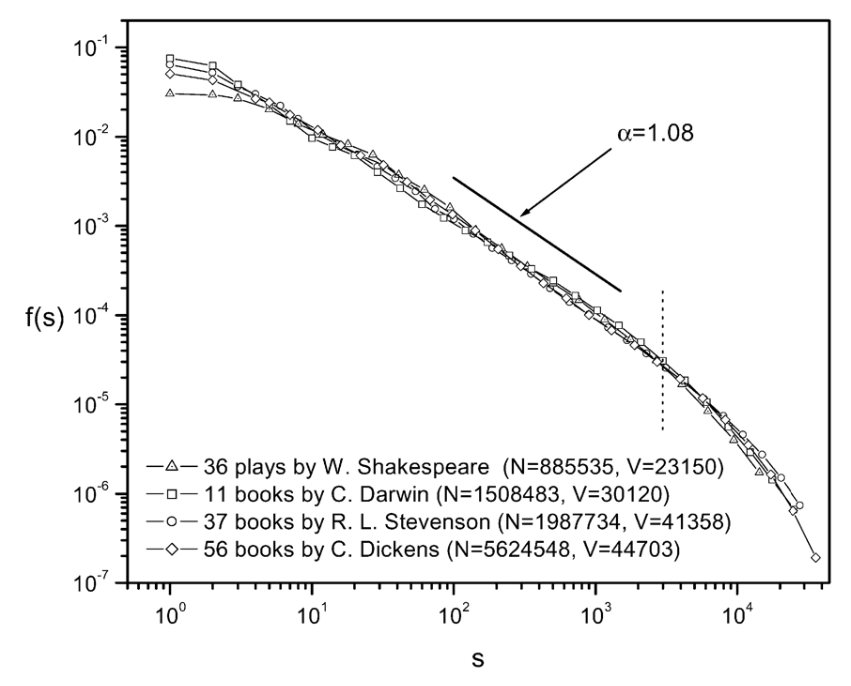
\includegraphics[scale=0.35]{figures/zipf-chart.png}
  %% \caption{Chart from \parencite{montemurro-2001-beyond-the-zipf} -``Frequency-rank distribution of words for four large text samples. In order to reveal individual variations these corpora are built with literary works of four different authors, respectively.  The vertical dash line is placed approximately where Zipf’s law ceases to hold''.}\label{fig:zipf-chart}
%% \end{figure}
%% As \textcite{montemurro-2001-beyond-the-zipf} note regarding the above figure, the relationship does not hold absolutely for lower frequency words. In their paper \parencite{montemurro-2001-beyond-the-zipf} they present a more detailed model capturing this variation. Their improved model is beyond the scope of this report but is illustrative of the difficulties of processing low-frequency words in particular, an issue we come across again later in this report.
%% 
The next concept is from the field of information theory and measures the amount of information revealed about a system when its outcome is partly decided. It is useful in embedding processes for quantifying how novel it is for two words to have co-occurred together (very frequent words like ``the'' are less novel partners to co-occur with than more domain-specific terms).

\begin{definition}[Pointwise Mutual Information]
  Given two discrete random variables with a joint distribution $P:X\times Y\to [0,1]$, such that the probability of $x$ and $y$ co-occurring is given by $P(x,y)$, the \emph{pointwise mutual information} of $x$ and $y$ is given by:
  \begin{equation}
    I(x,y)=\log\frac{P(x,y)}{P(x)P(y)}\label{eq:pmi}
  \end{equation}
\end{definition}

Pointwise mutual information is a measure of how much information about one random variable's value is gained, given that the value taken by the other is already known. For this reason it is natural to describe it in terms of conditional probabilities:
\begin{equation}
  I(x,y)=\log\frac{P(x\mid y)}{P(x)}
\end{equation}
This value happens to be symmetric with respect to $x$ and $y$:
\begin{equation}
  I(x,y)= \log\frac{P(x\mid y)P(y)}{P(x)P(Y)}\ =\ \log\frac{P(y\mid x)P(x)}{P(y)P(x)}=\log\frac{P(x, y)}{P(x)P(y)}
\end{equation}
which is why it is called the pointwise \emph{mutual} information.

If all outcomes in a joint distribution are equally likely, then learning the value of one of the variables does not give you any new information about the probability that the remaining variable takes any particular value. If the two are highly dependent on one another however, the outcome of one can be very informative about the probable outcomes for the other. This is the intuition which pointwise mutual information formalises.
\begin{example}[Pointwise mutual information] Given the definition we expect that for the two joint distributions ($P_1$, $P_2$, on $X$ and $Y$ shown in \autoref{tab:pmi1} and \autoref{tab:pmi2}), in the first case the pointwise mutual information for particular values (we choose $x_3$ and $y_3$) would be none, and in the second case would be positive. We calculate both below, referring to the first value $I_1$ and the second $I_2$.
  \phantom{para}\\\vspace{-3em}\par\hfill\allowbreak{}\\
  \hspace{-1.5em}
  \begin{minipage}{.5\textwidth}
  \vspace{0pt}
    \begin{center}\begin{tabular}{c R R !{\color{red}\vrule width 0.5pt} R !{\color{red}\vrule width 0.5pt} R r}
      \multicolumn{1}{c}   {  } & \multicolumn{1}{c} {$z_1$} & \multicolumn{1}{c} {$x_2$} & \multicolumn{1}{c} {$x_3$} & \multicolumn{1}{c} {$x_4$} & \multicolumn{1}{c} {}\\
      $y_1$ &  1/16  &  1/16  & 1/16 & 1/16    & \hspace{1em} 0.25\\
      $y_2$ &  1/16   &  1/16   & 1/16  & 1/16 & \hspace{1em} 0.25\\\hhline{~>{\arrayrulecolor{red}}----~}
      $y_3$ &  1/16  &  1/16  & 1/16 & 1/16    & \hspace{1em} 0.25\\\hhline{~>{\arrayrulecolor{red}}----~}
      $y_4$ &  1/16  &  1/16   & 1/16  & 1/16  & \hspace{1em} 0.25\\[0em]\\[-1em]
      \multicolumn{1}{c}   {} & \multicolumn{1}{c} {0.25} & \multicolumn{1}{c} {0.25} & \multicolumn{1}{c} {0.25} & \multicolumn{1}{c} {0.25} & \multicolumn{1}{c} {1}\\
    \end{tabular}\end{center}
  \captionof{table}{Case 1: $X$ and $Y$ with constant joint distribution $P_1$.}\label{tab:pmi1}
\end{minipage}
\hspace{1.4em}
\begin{minipage}{.5\textwidth}
  \vspace{0pt}
    \begin{center}\begin{tabular}{c R R !{\color{red}\vrule width 0.5pt} R !{\color{red}\vrule width 0.5pt} R r}
      \multicolumn{1}{c}   {  } & \multicolumn{1}{c} {$x_1$} & \multicolumn{1}{c} {$x_2$} & \multicolumn{1}{c} {$x_3$} & \multicolumn{1}{c} {$x_4$} & \multicolumn{1}{c} {}\\
      $y_1$ &  0.08  &  0.09  & 0.03 & 0.06    & \hspace{1em}0.26\\
      $y_2$ &  0.05   &  0.08   &  0.04 & 0.13 & \hspace{1em}0.30 \\\hhline{~>{\arrayrulecolor{red}}----~}
      $y_3$ &  0.11  &  0.03  & 0.03 & 0.06    & \hspace{1em}0.23 \\\hhline{~>{\arrayrulecolor{red}}----~}
      $y_4$ &  0.05  &  0.10   &  0.02 & 0.04  & \hspace{1em}0.21\\[0em]\\[-1em]
      \multicolumn{1}{c}   {} & \multicolumn{1}{c} {0.29} & \multicolumn{1}{c} {0.30} & \multicolumn{1}{c} {0.12} & \multicolumn{1}{c} {0.29} & \multicolumn{1}{c} {1}\\
    \end{tabular}\end{center}
  \captionof{table}{Case 2: $X$ and $Y$ with varied joint distribution $P_2$.}\label{tab:pmi2}
  \end{minipage}
  \phantom{para}\\[0.8em]
  \begin{align*}
    I_1(x_3,y_3)=\log\frac{P_1(x_3,y_3)}{P_1(x_3)P_1(y_3)}&=\log\frac{1/16}{0.25\cdot 0.25}\\
                                                          &=\log 1\ (= 0)\tag{first case}\\[1.5em]
    I_1(x_3,y_3)=\log\frac{P_2(x_3,y_3)}{P_2(x_3)P_2(y_3)}&=\log\frac{0.03}{0.23\cdot 0.12}\\
                                                          &=\log \frac{25}{23}\ (> 0)\tag{second case}
  \end{align*}
  You can see that the calculated PMI values conform with the intuition we described above.
  \vspace{0.0em}
\end{example}

\section{Tokenizing}
In this section we present a formal description of \emph{tokens}, the core unit upon which embedding algorithms operate on, in mathematical language. We did not find a formal description of tokens as mathematical elements like this in the literature -it is often assumed that a tokenized corpus is already prepared and understood- so we briefly present our own.

Since one of our aims in this report is to highlight the fact that many key ideas used to generate word spaces do not \emph{assume} that the objects being operated on are actually words (discussed in \nameref{chap:beyond-word-embeddings}), we thought a formal description of type of input generally expected by these algorithms would be a useful detail to specify.
\begin{definition}[Orthography]\label{def:orthography}
  An orthography is a finite set of symbols.
\end{definition}

\begin{example}\label{ex:orthographies}
  The sets:
  \begin{align}
    &\mathscr{O}_P=\{\mycirc[green], \mycirc[blue], \mycirc[red]\}\label{eq:dots-orthography}\\
    &\mathscr{O}_L=\{c\mid\text{$c$ is a letter, number or special character marked on \autoref{fig:uk-keyboard}}\}\label{eq:keyboard-orthography}
  \end{align}
  are both examples of orthographies.
\end{example}
\vspace{6pt}

\begin{figure}[ht]
 \centering
 \includesvg[width=0.9 \columnwidth]{figures/inkscape/uk-keyboard.svg}
 \caption{A standard uk keyboard layout}
 \label{fig:uk-keyboard}
\end{figure}

\begin{definition}[Document]
  A document $d$ is a finite sequence $c_0,c_1,\dots,c_n$ ($c\in\mathscr{O}$), where $\mathscr{O}$ is an orthography.
\end{definition}

\begin{example}[Dots Documents]\label{ex:doc-plato}
  The sequence of symbols:
  \[
    d_1=\fbox{\mycirc[red] \mycirc[green] \mycirc[blue] \mycirc[blue] \mycirc[red] \mycirc[blue] \mycirc[red] \mycirc[green] \mycirc[blue] \mycirc[green]}\label{eq:dots-document}
  \]
  is a document using orthography \eqref{eq:dots-orthography}.
\end{example}

\begin{example}[Plato Documents]\label{ex:doc-plato}
    Plain text versions of the complete works of Plato (English translations) are available at the \href{https://www.gutenberg.org/ebooks/author/93}{Project Gutenberg} website. These are examples of documents using keyboard orthography \ref{eq:keyboard-orthography} referenced above.
\end{example}

\begin{definition}[Word-Token]
  A word token $w$ is like a document -it is a sequence of symbols $c_0,c_1,\dots,c_n$ ($c\in\mathscr{O}$ from an orthography $\mathscr{O}$. The difference between a word token and a document is context: we call a sequence of symbols from an orthography a \emph{word token} when it is the output of a tokenizer (defined next).
\end{definition}

\begin{definition}[Tokenizer]
   A tokenizer $T$ is a function that maps a document to a sequence of word tokens; $T(d)=w_1,w_2,\dots,w_n$. The output is referred to as the 'tokenized' form of the document. We use the shorthand $W_d$ to refer to the tokenized document $T(d)$ when it is clear which tokenization has been used.\footnotemark.
\end{definition}
\footnotetext{Here we consider tokenization in an abstract sense essentially saying ``A tokenizer is a function that extracts tokens''. For a practical look at pre-processing see \nameref{chap:further-reading}.}

\begin{example}[Dots Document Tokenized]\label{ex:doc-plato}
  Using the tokenizing procedure: \emph{treat blue dots as token-deliminators}, the tokenization of document \eqref{eq:dots-document} yields:
  \begin{align}
    T(d_1)&=\fbox{\mycirc[red] \mycirc[green]}, \fbox{\mycirc[red]}, \fbox{\mycirc[red] \mycirc[green]}, \fbox{\mycirc[green]}\label{eq:dots-tokenized}\\
    &=W_{d_1}\nonumber
  \end{align}
\end{example}

\begin{example}[Simple Text Tokenizer]\label{ex:simple-tokenizer}
  In \autoref{alg:simple-tokenizer} we present a simple algorithm for tokenizing text which ignores a predefined list of special symbols, and identifies token-boundaries using predefined deliminator symbols.

  Setting {\sffamily ignore}$=("!", ".", ",", ";", ":", "'")$, and {\sffamily deliminators}$=("~")$, the following document:
  \begin{equation*}
    d_2=\text{\fbox{Predicting is difficult -especially about the future.}}
  \end{equation*}
  using the orthography \eqref{eq:keyboard-orthography} has the tokenized form:
  \begin{align}
    T(d_2)&=\text{\fbox{Predicting}}, \text{\fbox{is\vphantom{gt}}}, \text{\fbox{difficult\vphantom{gt}}}, \text{\fbox{-especially\vphantom{gt}}}, \text{\fbox{about\vphantom{gt}}}, \text{\fbox{the\vphantom{gt}}}, \text{\fbox{future\vphantom{gt}}}\label{eq:sentence-tokens}\\
    &=W_{d_2}\nonumber
  \end{align}
  Clearly the token \fbox{-especially} is not in the form an English speaker would transcribe if tasked with tokenizing the sentence by hand -but we use this example to highlight the difficulty of tokenizing: with this approach hyphenated expressions like ``brother-in-law'' will be correctly tokenized as single units, but in cases like \eqref{eq:sentence-tokens} mistakes are made. It is not possible to handle both cases correctly with our simple algorithm.
\end{example}

\begin{figure}[H]
  \centering
  \captionsetup{width=.91\linewidth}
  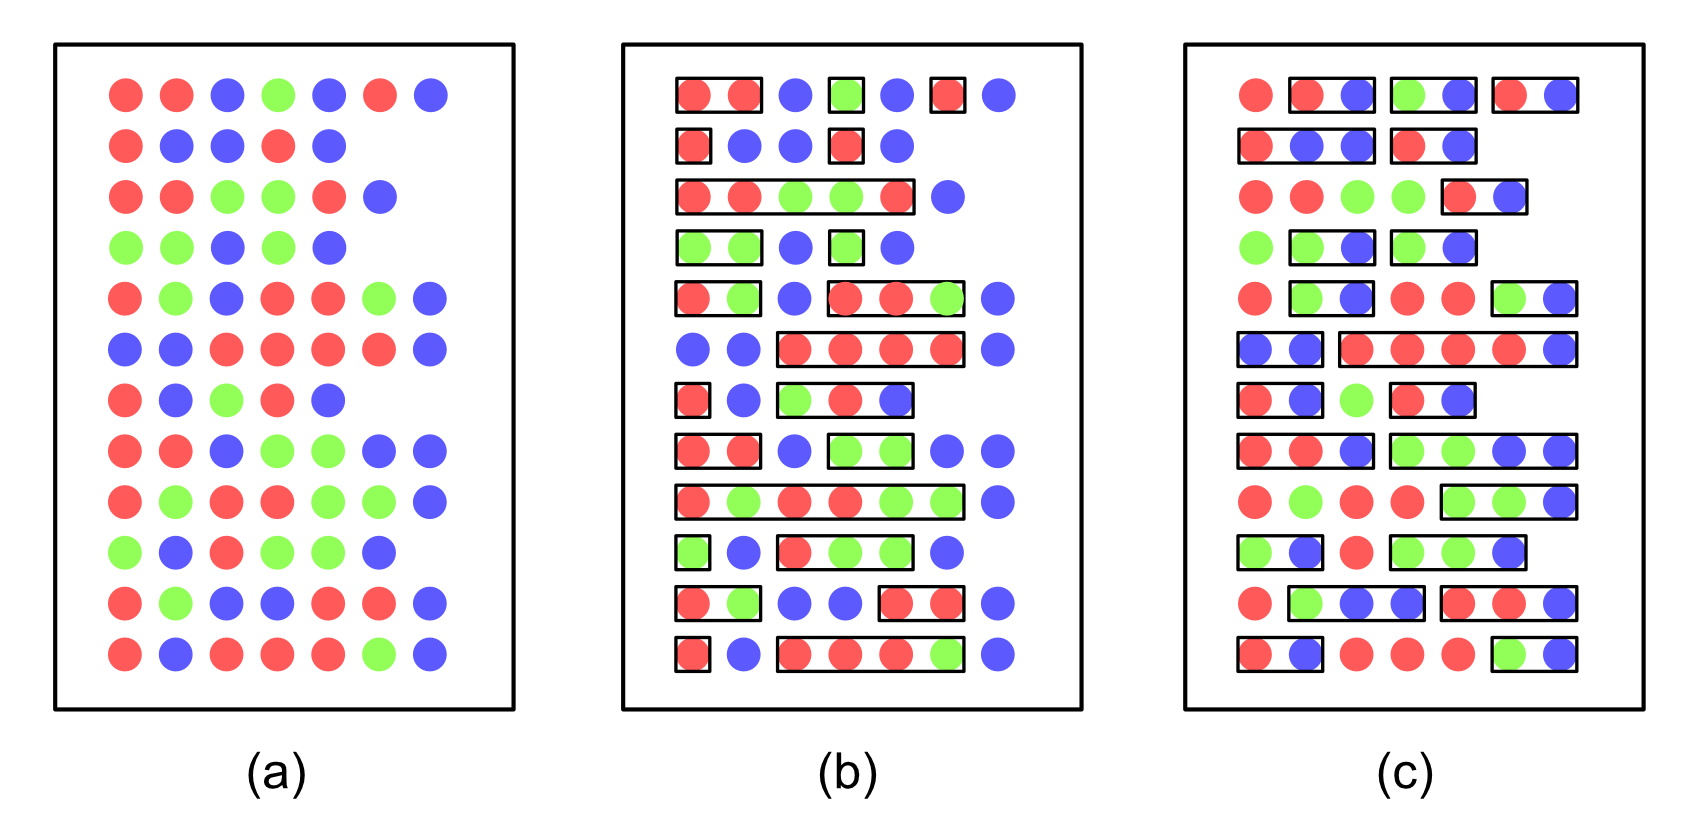
\includegraphics[scale=0.70]{figures/affinity-designer/tokens.png}
  \caption{Tokens identified by two different tokenizations, (b) \& (c), performed on the same document (a) (using the orthography~\eqref{eq:dots-orthography}). The tokenizer used in the case of (b) identifies tokens as sequences of red and green dots delimited by blue dots, and for (c) the tokenizer identified tokens as sequences of consecutive repeated symbols which are terminated by any number of blue dots.}\label{fig:dot-tokenizers}
\end{figure}
\par
\begin{algorithm}
  {\small
  \caption{Simple Text Tokenizer}\label{alg:simple-tokenizer}
  \SetNoFillComment{}
  \DontPrintSemicolon{}
  \SetKwData{Tokens}{tokens}
  \SetKwData{NextToken}{next\_token}
  \SetKwData{Ignore}{ignore}
  \SetKwData{Delim}{deliminators}
  \SetKwData{Doc}{document}
  \SetKwData{Symb}{symbol}
  \SetKwFunction{Append}{append}
  \SetKwFunction{List}{list}
  \SetKwFunction{Return}{return}
  \SetKwFunction{Preprocess}{preprocess}
  \SetKwInOut{Input}{input}\SetKwInOut{Output}{output}

  \Input{A list of symbols: \Doc, a list of ignored ``special'' symbols: \Ignore, and a list of deliminator symbols: \Delim}
  \Output{A list of word tokens: \Tokens}
  \BlankLine

  \Tokens $\leftarrow$ \List{}\;
  \NextToken $\leftarrow$ \List{}\;
  \tcc{Go through the document one symbol at a time, skipping special characters, and adding \NextToken to \Tokens when a deliminator is reached}
  \For{\Symb in \Doc}{
    \uIf{\Symb is in \Delim}{
      \tcc{Add \NextToken to \Tokens if \NextToken only if it contains symbols}
      \uIf{\NextToken is not empty}{
        \Tokens$\leftarrow$ \Append{\NextToken, \Tokens}\;
        \NextToken$\leftarrow$ \List{}\;
      }
      \Else{
        \tcc{Keep parsing symbols to add to \NextToken until the next deliminator is reached}
      }
    }
    \uElseIf{\Symb is in \Ignore}{
      \tcc{Ignore this symbol}
    }
    \Else{
      \tcc{Add this symbol to the \NextToken variable}
      \NextToken$\leftarrow$ \Append{\Symb, \NextToken}\;
    }
  }
  \Return{\Tokens}
  }
\end{algorithm}
\par
We have described tokenization for orthographies of letter-based and dot-based documents but of course there are many other possibilities, for example tokenizing musical notation by delimiting tokens at bar-boundaries.

\begin{definition}[Corpus]
  A corpus $C$ is a finite set of documents $\{d_1, d_2,\dots,d_n\}$, $n\in\mathbb{N}$.
\end{definition}

\begin{example}[Plato Corpus]\label{ex:corp-plato}
  The complete works of Plato in plain-text form, referenced in \autoref{ex:doc-plato} is an example of a corpus.
\end{example}

\begin{definition}[Vocabulary]
  The vocabulary of a tokenized document $W_d$ is the set of unique word tokens in the tokenization of that document; $V(W_d)=\{w\mid w\in\, \text{the sequence $W_d$}\}$. The vocabulary of a corpus is the union of the vocabularies of each document in that corpus; $V(C)=V(W_{d_1})\cup V(W_{d_2})\cup \dots\cup V(W_{d_n})$.
\end{definition}

\begin{definition}[$\#$ Operator]
  The $\#$ symbol, used preceding a set or a sequence, denotes ``the number of elements in''. $\#W_d$ denotes the number of tokens in the tokenized form of document $d$ then, and $\#V(W_d)$ denotes the vocabulary size of document $d$.
\end{definition}

\begin{example}[Dots Document Properties]
  The vocabulary of the tokenized document \eqref{eq:dots-tokenized} is:
  \begin{align*}
    V(W_{d_1})&=V(\fbox{\mycirc[red] \mycirc[green]}, \fbox{\mycirc[red]}, \fbox{\mycirc[red] \mycirc[green]}, \fbox{\mycirc[green]})\\
              &=\{\fbox{\mycirc[red] \mycirc[green]}, \fbox{\mycirc[red]}, \fbox{\mycirc[green]}\}
  \end{align*}
  The number of tokens (the word count) for this document is: $\#W_{d_1}=4$ and the vocabulary size is $\#V(W_{d_1})=3$
\end{example}

\begin{example}[Plato Document Sizes]
  Word token counts and vocabulary sizes for a selection Plato documents from~\ref{ex:doc-plato}, tokenized using a variation of the simple tokenizer\footnotemark described by \autoref{alg:simple-tokenizer}, are listed here:\\[-1em]
  \begin{center}
  \captionsetup{width=.91\linewidth}
    \begin{tabular}{c r r r r r r}
      \toprule
      \multicolumn{1}{c}{Attribute$\quad$} &
      \multicolumn{6}{c}{Document ($d$)} \\

      \cmidrule(lr){2-7}
      &
      $\texttt{laws}$ &
      $\texttt{republic}$ &
      $\texttt{cratylus}$ &
      $\texttt{meno}$ &
      $\texttt{apology}$ &
      $\texttt{crito}$ \\
      \midrule
      $\#W_d$ & 140,406 & 118,283 & 23,883 & 12,716 & 11,392 & 5,332\\
      $\#V(W_d)$ & 8,100 & 8,105 & 2,963 & 1,493 & 1,789 & 1,030\\
      \bottomrule
    \end{tabular}
    \captionof{table}{Number of Word Tokens \& Vocabulary Sizes of a selection of Documents in the Plato Corpus (\autoref{ex:corp-plato})}
    \end{center}
\end{example}
\footnotetext{The code used to produce this table, and other examples using this data set, is available on \href{https://github.com/joelstrouts/degree-project}{Github}.}

\begin{example}[Plato Corpus Size]
  The complete Plato corpus (\ref{ex:corp-plato}) consists of 25 documents and, each tokenized the same way as before, has the word count $\sum_{d\in C_P}\#W_d=670,936$ and the vocabulary size $\#V(C_P)=19,432$.
\end{example}
\noindent
These are the essential mathematical objects which are used to construct co-occurrence matrices as we describe in the following chapter.

\section{Similarity Measure}
There are many possible measures of similarity for comparing two vectors, but in the word embedding domain by far the most prevalent is the cosine similarity. We present only this method, but suggest reading \textcite{bullinaria-2007-extracting-semantic} for a discussion and comparison of other distance measuring approaches.

\begin{definition}[Cosine Similarity]
  Give two non-zero vectors $\bf{x}$ and $\bf{y}$, the cosine similarity between these two vectors is given by:
  \begin{equation}
    \operatorname{sim}(\bf{x}, \bf{y})=\frac{\bf{x}\cdot\bf{y}}{||\bf{x}||||\bf{y}||}
  \end{equation}
  where $\bf{x}\cdot\bf{y}$ is the dot product of $\bf{x}$ and $\bf{y}$ and $||\bf{v}||$ is the norm of $\bf{x}$.
  This formula is derived from the dot product formula: $\bf{x}\cdot\bf{y}=||\bf{x}||||\bf{y}||\cos\theta$.
\end{definition}

%%% Local Variables:
%%% mode: latex
%%% TeX-master: "../main"
%%% End:

% ++ semantic relatedness (syntagmatic.. paradigmatic .. etc.)
% ++ distributive properties??
% ++++ zipfs law
% ++++ bayes? whatever
% ++ measures of similarity
% ++ terminology/definitions
\chapter{Count Models}\label{chap:count-models}
\section{Cooccurrence Matrix Types}
\section{Smoothing}
\section{Dimensionality Reduction}

% ++ types of cooccurrence matrix
% ++ smoothing
% ++ dimension reduction
% ++ computation
% ++ comparison with other models
\chapter*{Further Reading}\label{chap:further-reading}
\addcontentsline{toc}{chapter}{Further Reading}
In this section we briefly identify key resources used in the writing of this report and suggest other material for further reading, in particular regarding the practical application of embedding algorithms.

\begin{infobox}{Selected topics and references}{\small
  \paragraph{Key references} These resources have been invaluable in writing this report:\hspace{1.4em}
  \begin{enumerate}
    \item On words: \emph{\citetitle{halliday-2004-lexicology, dixon02-word}} \parencite{halliday-2004-lexicology, dixon02-word},\vspace{-0.5em}
    \item On Count models: \emph{\citetitle{turney10-from-frequen-to-meanin, sahlgreen-2006-the-word-space-model}} \parencite{turney10-from-frequen-to-meanin, sahlgreen-2006-the-word-space-model},\vspace{-0.5em}, 
    \item An overview of embedding methods: \emph{\citetitle{wang-2019-evaluating, almeida19-word-embed}} \parencite{wang-2019-evaluating, almeida19-word-embed}
    \end{enumerate}
  \paragraph{Pre-processing}
  Although we discussed tokenization in this report we did not discuss the more general problem of text pre-processing. Purposes of pre-processing can be lemmatization (replacing words with their ``lemma'' form i.e., looks$\rightarrow$look and running$\rightarrow$run), lowercasing, stop-word removal, multiword grouping (identifying multi-part grammatical words as single tokens). Suggested reading:
  \begin{enumerate}
    \item \emph{\citetitle{uysal-2014-the-impact-of-preprocessing}} \parencite{uysal-2014-the-impact-of-preprocessing},\vspace{-0.5em}
    \item \emph{\citetitle{camacho-collados17-role-text-prepr-neural-networ-archit}} \parencite{camacho-collados17-role-text-prepr-neural-networ-archit}.
  \end{enumerate}
  \paragraph{Bias}\label{para:bias}
  Since embedding algorithms do not understand language, they just identify statistical regularities in corpora, if that training data contains bias then that bias will be represented (or even amplified) in the embedding output. Suggested reading:
  \begin{enumerate}
    \item \emph{\citetitle{caliskan-2017-semantics-derived}} \parencite{caliskan-2017-semantics-derived},\vspace{-0.5em}
    \item \emph{\citetitle{bolukbasi16-man-is-to-comput-progr}} \parencite{bolukbasi16-man-is-to-comput-progr}.
  \end{enumerate}
}\end{infobox}
% ++ preprocessing
% ++ bias
\chapter*{Conclusion}\label{chap:conclusion}\label{conclusion}
\addcontentsline{toc}{chapter}{Conclusion}
Word embeddings are an essential tool in the NLP toolbox -they are ``a standard component of most state-of-the-art NLP architectures'' \parencite{peters18-deep-contex-word-repres}. They enable many systems which have to interact with language in some capacity do so more `intelligently'. In this report we have tried to describe the problems which make the creation of \emph{truly} intelligent word embeddings more difficult. Engineering better methods for representing language requires understanding what written language \emph{is} and how it performs its function. Cutting edge methods like that of \textcite{devlin-etal-2019-bert}, which incorporate an element of language modelling, will likely become the standard for this reason. Despite this, it is remarkable how much semantic information is encoded by even the most simple models, applicable to any type of sequenced data because of their \emph{lack} of assumptions. The core idea behind word embeddings, \emph{the distributional hypothesis}, is a powerful one. Finally, for practitioners of these methods the \nameref{para:bias} aspect is essential to consider: embedded representations say nothing `objective' about the concepts they represent, they are only a reflection of their training data. This is not a shortcoming of the methods used, it should just inform their manner of application -a good use of this bias-capturing nature of embeddings is for studying bias itself, see \parencite{garg-2018-word-embeddings-quantify} for such an investigation.

\makebibliography
\end{document}
